% Research Assistant runtime architecture (editable source of the shared figure).
%
% Rebuild from the project root; build in a temporary folder so .aux/.log files
% never land in the repository:
%   pdflatex -interaction=nonstopmode -output-directory=<tmp> docs/figures/architecture.tex
%   copy <tmp>/architecture.pdf to docs/figures/architecture.pdf
%   pdftoppm -png -r 300 -singlefile docs/figures/architecture.pdf docs/figures/architecture
% Overleaf also compiles this file with pdfLaTeX.
%
% Solid arrows are calls from caller to callee; the circled numbers give their
% order in one `ask` request. Dashed arrows are configuration, local files or
% output. Paths in the layer tabs are relative to src/researcher/.
% docs/architecture.md explains each box; keep both in sync with the code.
\documentclass[tikz,border=4pt]{standalone}
\usepackage[T1]{fontenc}
\usepackage{courier}
\usepackage[scaled=0.95]{helvet}
\renewcommand{\familydefault}{\sfdefault}
\usetikzlibrary{arrows.meta,backgrounds,calc,fit,shapes.geometric}

\definecolor{ink}{HTML}{1A202C}
\definecolor{edge}{HTML}{4A5568}
\definecolor{userfill}{HTML}{EDF2F7}
\definecolor{entryfill}{HTML}{EBF8FF}\definecolor{entryline}{HTML}{3182CE}
\definecolor{corefill}{HTML}{F0FFF4}\definecolor{coreline}{HTML}{38A169}
\definecolor{concfill}{HTML}{FAF5FF}\definecolor{concline}{HTML}{805AD5}
\definecolor{svcfill}{HTML}{FFFAF0}\definecolor{svcline}{HTML}{DD6B20}
\definecolor{storefill}{HTML}{F7FAFC}\definecolor{storeline}{HTML}{718096}
\definecolor{aifill}{HTML}{FFF5F5}\definecolor{ailine}{HTML}{C53030}
\definecolor{extfill}{HTML}{EDF2F7}\definecolor{extline}{HTML}{A0AEC0}
\definecolor{notefill}{HTML}{FEFCBF}\definecolor{noteline}{HTML}{B7791F}
\definecolor{filefill}{HTML}{E2E8F0}

\newcommand{\dotsep}{\,\textperiodcentered\,}

\begin{document}
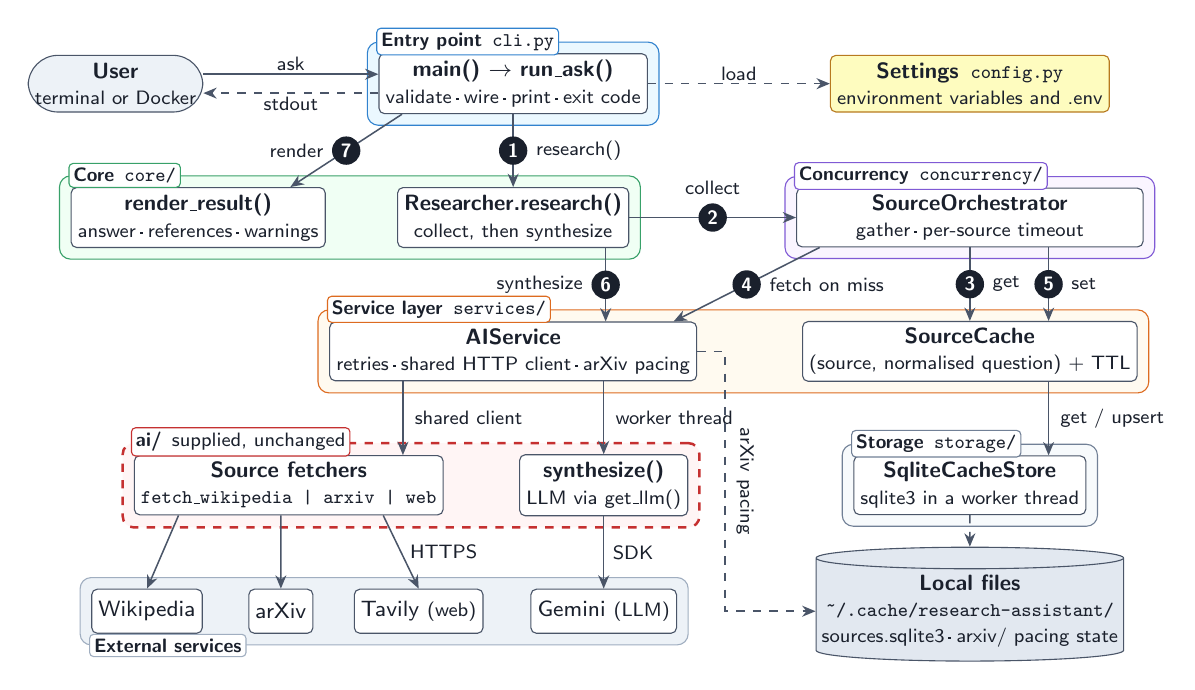
\begin{tikzpicture}[
  comp/.style={draw=edge, fill=white, rounded corners=2pt, align=center,
    font=\footnotesize, text=ink, inner sep=2.4pt, minimum height=7.2mm},
  ext/.style={comp, minimum height=5.6mm},
  layerbox/.style={draw=#1, rounded corners=4pt, inner sep=4pt},
  tab/.style={draw=#1, fill=white, rounded corners=1.5pt, font=\scriptsize,
    text=ink, inner sep=1.6pt},
  call/.style={-{Stealth[length=1.7mm,width=1.4mm]}, draw=edge, line width=0.55pt},
  aux/.style={call, dashed},
  stepno/.style={circle, fill=ink, text=white, font=\scriptsize\bfseries,
    inner sep=0pt, minimum size=3.6mm},
  note/.style={font=\scriptsize, text=ink, inner sep=1pt},
]
% ---- Band 1: user and entry point ------------------------------------------
\node[comp, fill=userfill, rounded corners=3.8mm] (user) at (1.35,7.55)
  {\textbf{User}\\{\scriptsize terminal or Docker}};
\node[comp] (cli) at (6.4,7.55)
  {\textbf{main() $\rightarrow$ run\_ask()}\\{\scriptsize validate\dotsep wire\dotsep print\dotsep exit code}};
\node[comp, fill=notefill, draw=noteline] (settings) at (12.2,7.55)
  {\textbf{Settings}\enspace{\scriptsize\ttfamily config.py}\\{\scriptsize environment variables and .env}};

% ---- Band 2: core logic and concurrency ------------------------------------
\node[comp] (render) at (2.4,5.85)
  {\textbf{render\_result()}\\{\scriptsize answer\dotsep references\dotsep warnings}};
\node[comp] (researcher) at (6.4,5.85)
  {\textbf{Researcher.research()}\\{\scriptsize collect, then synthesize}};
\node[comp, minimum width=44mm] (orchestrator) at (12.2,5.85)
  {\textbf{SourceOrchestrator}\\{\scriptsize gather\dotsep per-source timeout}};

% ---- Band 3: service layer --------------------------------------------------
\node[comp] (aiservice) at (6.4,4.15)
  {\textbf{AIService}\\{\scriptsize retries\dotsep shared HTTP client\dotsep arXiv pacing}};
\node[comp] (cache) at (12.2,4.15)
  {\textbf{SourceCache}\\{\scriptsize (source, normalised question) + TTL}};

% ---- Band 4: supplied ai/ package and storage -------------------------------
\node[comp] (fetchers) at (3.55,2.45)
  {\textbf{Source fetchers}\\{\scriptsize\ttfamily fetch\_wikipedia | arxiv | web}};
\node[comp] (synthesize) at (7.55,2.45)
  {\textbf{synthesize()}\\{\scriptsize LLM via get\_llm()}};
\node[comp] (store) at (12.2,2.45)
  {\textbf{SqliteCacheStore}\\{\scriptsize sqlite3 in a worker thread}};

% ---- Band 5: external services and local files -----------------------------
\node[ext] (wiki) at (1.75,0.85) {Wikipedia};
\node[ext] (arxiv) at (3.45,0.85) {arXiv};
\node[ext] (tavily) at (5.2,0.85) {Tavily {\scriptsize(web)}};
\node[ext] (gemini) at (7.55,0.85) {Gemini {\scriptsize(LLM)}};
\node[cylinder, shape border rotate=90, aspect=0.07, draw=edge, fill=filefill,
      align=center, font=\footnotesize, text=ink, inner sep=2pt] (files) at (12.2,0.85)
  {\textbf{Local files}\\{\scriptsize\ttfamily \textasciitilde/.cache/research-assistant/}\\{\scriptsize sources.sqlite3\dotsep arxiv/ pacing state}};

% ---- Layer boxes and tabs ---------------------------------------------------
\begin{scope}[on background layer]
  \node[layerbox=entryline, fill=entryfill, fit=(cli)] (entrybox) {};
  \node[layerbox=coreline, fill=corefill, fit=(render)(researcher)] (corebox) {};
  \node[layerbox=concline, fill=concfill, fit=(orchestrator)] (concbox) {};
  \node[layerbox=svcline, fill=svcfill, fit=(aiservice)(cache)] (svcbox) {};
  \node[layerbox=storeline, fill=storefill, fit=(store)] (storebox) {};
  \node[layerbox=ailine, fill=aifill, dashed, line width=0.9pt, fit=(fetchers)(synthesize)] (aibox) {};
  \node[layerbox=extline, fill=extfill, fit=(wiki)(arxiv)(tavily)(gemini)] (extbox) {};
\end{scope}
\node[tab=entryline, anchor=west] at ($(entrybox.north west)+(0.12,0)$)
  {\textbf{Entry point}\enspace\texttt{cli.py}};
\node[tab=coreline, anchor=west] at ($(corebox.north west)+(0.12,0)$)
  {\textbf{Core}\enspace\texttt{core/}};
\node[tab=concline, anchor=west] at ($(concbox.north west)+(0.12,0)$)
  {\textbf{Concurrency}\enspace\texttt{concurrency/}};
\node[tab=svcline, anchor=west] at ($(svcbox.north west)+(0.12,0)$)
  {\textbf{Service layer}\enspace\texttt{services/}};
\node[tab=storeline, anchor=west] at ($(storebox.north west)+(0.12,0)$)
  {\textbf{Storage}\enspace\texttt{storage/}};
\node[tab=ailine, anchor=west] at ($(aibox.north west)+(0.12,0)$)
  {\textbf{ai/}\enspace supplied, unchanged};
\node[tab=extline, anchor=west] at ($(extbox.south west)+(0.12,0)$)
  {\textbf{External services}};

% ---- Calls and data movement ------------------------------------------------
\draw[call] ($(user.east)+(0,0.12)$) -- node[note, above] {ask} ($(cli.west)+(0,0.12)$);
\draw[aux] ($(cli.west)+(0,-0.12)$) -- node[note, below] {stdout} ($(user.east)+(0,-0.12)$);
\draw[aux] (cli) -- node[note, above] {load} (settings);

\draw[call] (cli.south -| researcher) -- node[stepno] {1}
  node[note, right=7pt] {research()} (researcher.north);
\draw[call] (researcher) -- node[stepno] {2} node[note, above=7pt] {collect} (orchestrator);
\draw[call] (orchestrator.south) -- node[stepno] {3}
  node[note, right=7pt] {get} (cache.north);
\draw[call] ($(orchestrator.south west)+(0.3,0)$) -- node[stepno] {4}
  node[note, right=7pt] {fetch on miss} ($(aiservice.north east)+(-0.3,0)$);
\draw[call] ($(orchestrator.south)+(1.0,0)$) -- node[stepno] {5}
  node[note, right=7pt] {set} ($(cache.north)+(1.0,0)$);
\draw[call] ($(researcher.south east)+(-0.3,0)$) -- node[stepno] {6}
  node[note, left=7pt] {synthesize} ($(researcher.south east |- aiservice.north)+(-0.3,0)$);
\draw[call] ($(cli.south west)+(0.3,0)$) -- node[stepno] {7}
  node[note, left=7pt] {render} ($(render.north east)+(-0.45,0)$);

\coordinate (fetchcol) at (5.0,0);
\draw[call] (aiservice.south -| fetchcol) -- node[note, right=3pt] {shared client}
  (fetchers.north -| fetchcol);
\draw[call] (aiservice.south -| synthesize) -- node[note, right=3pt] {worker thread}
  (synthesize.north);
\draw[aux] (aiservice.east) -- ++(0.35,0) coordinate (bend)
  -- node[note, sloped, above=3pt, pos=0.5] {arXiv pacing} (bend |- files.west) -- (files.west);
\draw[call] ($(cache.south)+(1.0,0)$) -- node[note, right=3pt] {get / upsert}
  ($(store.north)+(1.0,0)$);
\draw[aux] (store) -- (files);

\draw[call] ($(fetchers.south)+(-1.4,0)$) -- (wiki.north);
\draw[call] ($(fetchers.south)+(-0.1,0)$) -- (arxiv.north);
\draw[call] ($(fetchers.south)+(1.2,0)$) -- node[note, right=2pt] {HTTPS} (tavily.north);
\draw[call] (synthesize.south) -- node[note, right=2pt] {SDK} (gemini.north);
\end{tikzpicture}
\end{document}
